% !TEX root = journal.tex
\section{Introduction}
% Computer Society journal papers do something a tad strange with the very
% first section heading (almost always called "Introduction"). They place it
% ABOVE the main text! IEEEtran.cls currently does not do this for you.
% However, You can achieve this effect by making LaTeX jump through some
% hoops via something like:
%
%\ifCLASSOPTIONcompsoc
%  \noindent\raisebox{2\baselineskip}[0pt][0pt]%
%  {\parbox{\columnwidth}{\section{Introduction}\label{sec:introduction}%
%  \global\everypar=\everypar}}%
%  \vspace{-1\baselineskip}\vspace{-\parskip}\par
%\else
%  \section{Introduction}\label{sec:introduction}\par
%\fi
%
% Admittedly, this is a hack and may well be fragile, but seems to do the
% trick for me. Note the need to keep any \label that may be used right
% after \section in the above as the hack puts \section within a raised box.



% The very first letter is a 2 line initial drop letter followed
% by the rest of the first word in caps (small caps for compsoc).
% 
% form to use if the first word consists of a single letter:
% \IEEEPARstart{A}{demo} file is ....
% 
% form to use if you need the single drop letter followed by
% normal text (unknown if ever used by IEEE):
% \IEEEPARstart{A}{}demo file is ....
% 
% Some journals put the first two words in caps:
% \IEEEPARstart{T}{his demo} file is ....
% 
% Here we have the typical use of a "T" for an initial drop letter
% and "HIS" in caps to complete the first word.
\IEEEPARstart{T}{he}   main purpose of graphics is to summarize data and present them in a way that readers are able to extract the main message quickly and with a minimum of distortion. Tufte  coined the amount of distortion the \emph{Lie-Factor} \citep[p. 57--69]{tufte} of a chart, defined as the ratio of the size of an effect shown in a chart in comparison to the size of the same effect in the data. Ideally, this ratio is one. 

As designers of charts we have to be aware of the innate or culturally imposed perceptual limitations of our audience. This gives rise to another kind of distortion that may lead to effects similar to a Lie-Factor: while the physical quantity drawn in the chart might  perfectly reflect the  size of an effect in the data, an observer might intuitively interpret another property of the geometrical object, leading to distorted, if not altogether wrong, conclusions. 

%

%% from http://what-when-how.com/sociology/statistical-graphics/
%The effectiveness of statistical graphs is rooted in the remarkable ability of people to apprehend, process, and remember pictorial information. The human visual system, however, is subject to distortion and illusion, processes that can affect the perception of graphs. Good graphical design can minimize and counteract the limitations of human vision. In Figure 9, for example, it appears that the difference between the hypothetical import and export series is changing when this difference actually is constant (cf., Playfair?s time series graph in Figure 2 a). 

As an example for the phenomenon we concentrate on in this paper, we refer you to the top chart in  figure  \ref{playfair}. 
This chart shows Playfair's  visualization of the balance of trade between England and the East Indies as published in his Commercial and Political Atlas, 1786 \cite{playfair, playfair2}. 

When asked to sketch out the difference between imports and exports \citep{cleveland:1984}, observers very often miss the steep rise in the difference between the lines starting just before 1760 (see the chart at the bottom for the actual difference between imports and exports).

This phenomenon  is known and widely discussed in statistical graphics literature \citep{wainer:2000, robbins:2005}. The line width illusion is due to our  tendency to assess distance between curves as the minimal (orthogonal) distance rather than the  vertical distance -- see sketch \ref{fig:linewidth}.


In the perception literature, this phenomenon is known as part of a group of geometrical optical misperceptions of a context-sensitive nature classified as M\"uller-Lyer illusions \citep{day:1991}. Interestingly, there seems to be a general agreement that this illusion exists, but a quantification of it is curiously absent from the literature.


%XXX Why don't we mention mosaics? - I don't want to, but we need a better reason

\begin{figure}
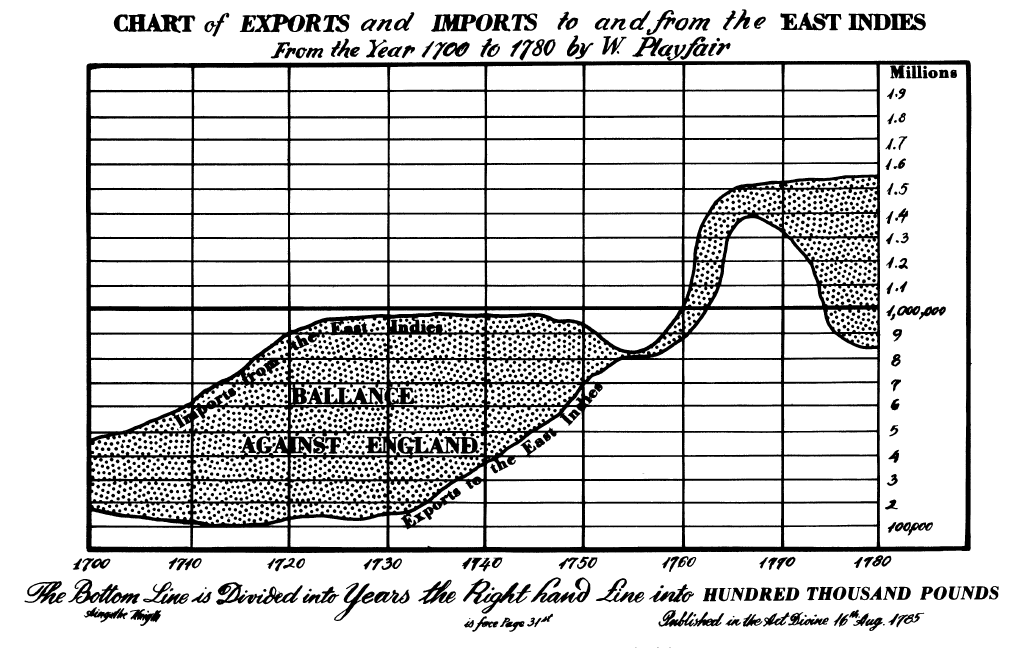
\includegraphics[width=.9\linewidth]{playfair_east_indies_gross}
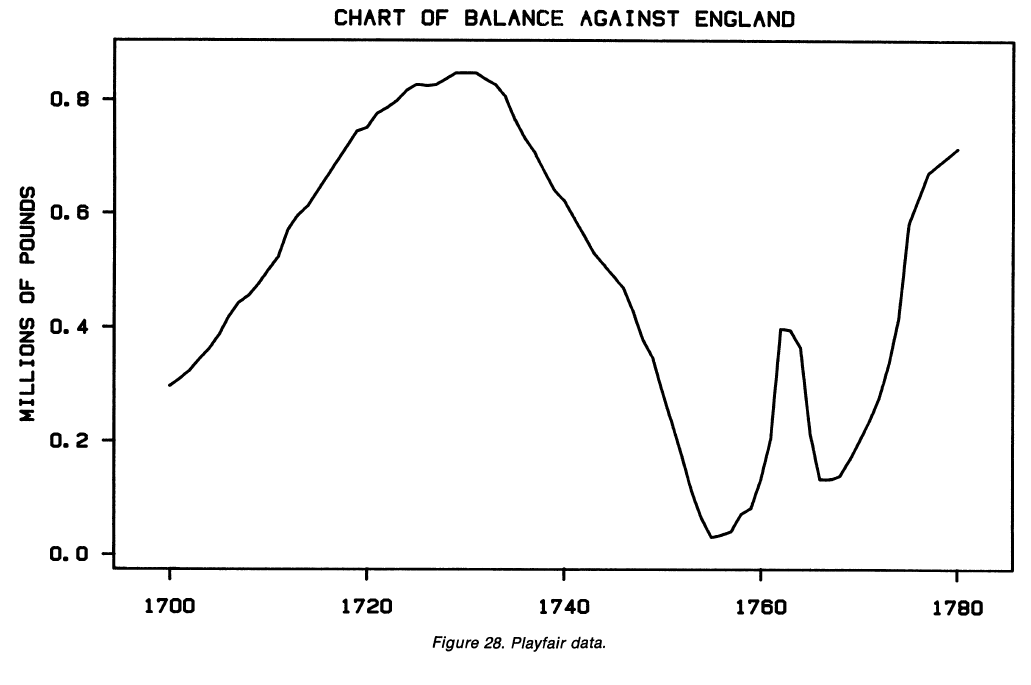
\includegraphics[width=.8\linewidth, height=.4\linewidth]{playfair_differenz_cleveland}
\caption{Playfair's chart from the Commercial and Political Atlas, 1786 (above). The sketch below shows  the difference between the lines for export and import - the steep rise in the difference around 1760  comes as a surprise to many onlookers.  }
\label{playfair}
\end{figure}

%Figure \ref{sine-illusion} shows a screen shot of applet displaying the sine illusion. The sine illusion is closely related to the line width phenomenon -- the line segments in the are of the steepest slope of the sine curve appear to be the shortest: ``The illusion is explained in terms of a perceptual compromise between the vertical extent and the greater overall dimensions of the section at the turn of the sine-wave figure and is thereby held to be the same in principle as the M\"uller-Lyer illusion." \citep{day:1991}.
%M Bach's applet \citep{bach} gives the option to compensate the line length manually for its perceived shortcoming. The amount of compensation chosen turns out to be highly dependent on both the length of the vertical line segments and the amplitude of the sine function. The amplitude directly affects the slope -- the steeper  the slope the more compensation is necessary, see section \ref{distortion}  for a more detailed discussion and some results from a user study.
%
%
%\begin{figure}
%\centering 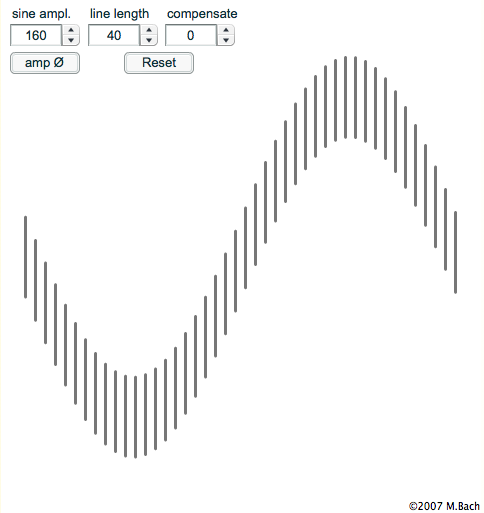
\includegraphics[width=.75\linewidth]{sine-illusion}
%\caption{Screenshot of an applet by M Bach \citep{bach} showing an example of a sine illusion. The applet is giving the possibility for compensating the line lengths in the regions with the highest slope. }
%\label{sine-illusion}
%\end{figure}

In this paper we focus on the use of parallel coordinate plots \citep{pcp:1885, inselberg:1985, wegman:1990} for categorical data and the perceptual implications this has.

We will first give an overview of  charts commonly used for displaying associations between categorical variables within the framework of parallel coordinate plots, and then discuss their performance with respect to the line width illusion.


\subsection{Parallel Set Plots}


Parallel Sets have been introduced by R Kosara \citep{kosara:2006} as a way to visualize categorical data within the framework of parallel coordinate plots  and have by now spread into main media, see e.g. the article on decision making in the BBC \citep{bbc:2009}. 

%XXX Description of parallel sets - and example
Figure \ref{question1a} gives an example for a parallel sets plot of the Titanic data \citep{dawson:1995}. The top bar shows classification of people on board according to their status as crew member and passengers. Passengers are further divided into first, second or third class. The bottom bar shows survival  as yes and no. Between the bars lines are drawn to visualize the relationship between class membership and  survival. Based on the proportion of survivor and non survivors bands are drawn from each class, the (horizontal) width of which is proportional to the number of people they represent. 

This definition makes parallel sets unfortunately a victim of the line width illusion, which in extreme cases can be so severe as to lead the user to wrong conclusions about the displayed data.  Section \ref{distortion}  shows more details on the strength of this illusion.


\subsection{Strength of the Linewidth Illusion}\label{distortion}
\begin{figure}[hbtp]
\centering
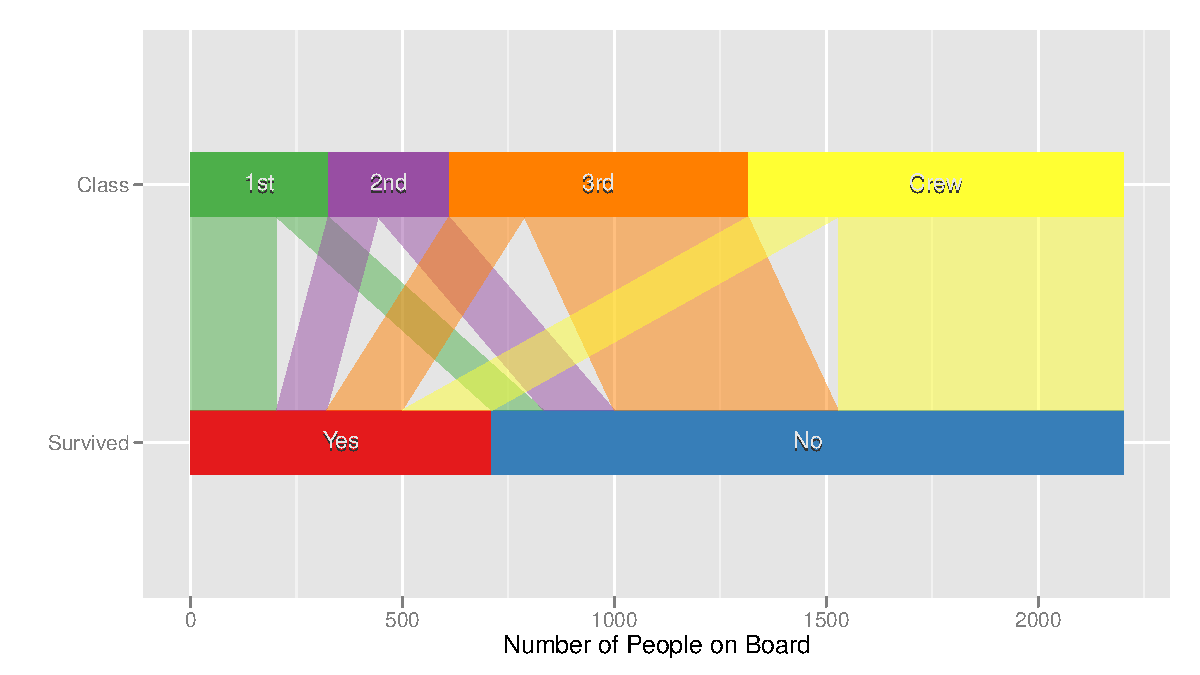
\includegraphics[width=.9\linewidth]{images/parset-titanic}
\caption{\label{question1a} Parallel sets plot showing Survival by Class for the Titanic Data. }
\end{figure}

\begin{figure}[hbtp]
\begin{center}
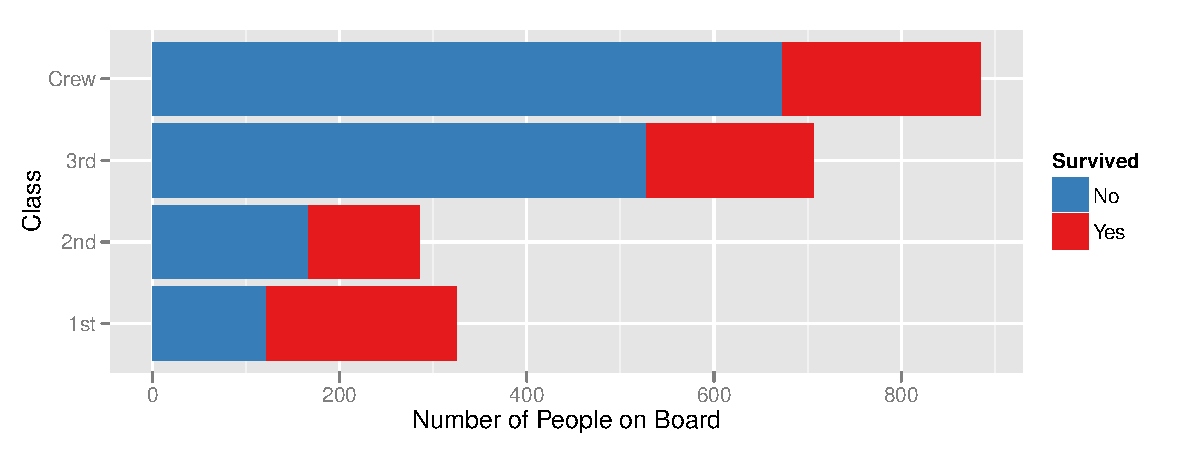
\includegraphics[width=.8\linewidth]{images/bar1-titanic}
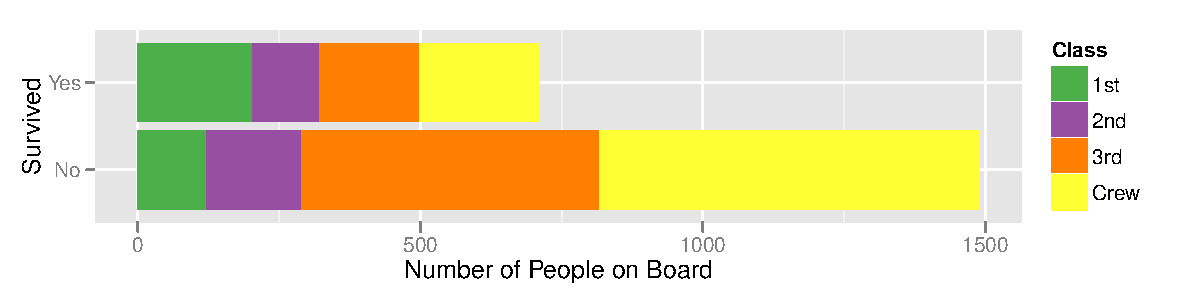
\includegraphics[width=.8\linewidth]{images/bar2-titanic}
\end{center}
\caption{\label{question1b} Barcharts showing Survival by Class for the Titanic Data.}
\end{figure}



In a preliminary survey participants were asked to order class  levels according to the number of survivors (from highest to lowest) based on  either the parallel sets plot of figure \ref{question1a} or the set of two barcharts in figure \ref{question1b} showing the same data.  The actual number of survivors by class are
%
\begin{center}
\begin{tabular}{rrrrr}
& Crew & 1st & 2nd & 3rd \\ \hline
Survivors & 212 & 203 & 118 & 178\\
Non-Survivors & 673 & 122 & 167 &  528  
\end{tabular}
\end{center}


% latex table generated in R 2.15.0 by xtable 1.7-0 package
% Sat May 12 20:04:08 2012
\begin{table}[ht]
\begin{center}
\begin{tabular}{rrrl}
  \hline
 & barcharts & parallel sets & Correct \\ 
  \hline
 1st, 3rd, Crew,  2nd & 0 & 8 &  \\ 
  1st, 2nd, Crew, 3rd & 0 & 4 &  \\ 
 1st, Crew, 3rd, 2nd & 3 & 1 &  \\ 
  Crew, 1st, 3rd, 2nd & 7 & 0 & * \\ 
  Crew, 2nd, 3rd, 1st & 1 & 0 &  \\ 
  Crew, 3rd, 2nd, 1st & 1 & 0 &  \\ 
   \hline
(all) & 12 & 13 &  \\ 
   \hline
\end{tabular}
\caption{Overview of survey results: 7 out of 12 participants facing the barchart picked the correct order of `Crew, 1st, 3rd, 2nd' (highest number of survivors to lowest). None of the 13 participants evaluating the parallel set plot picked the correct result. }
\label{tab:results}
\end{center}
\end{table}


%  , , qid = 2
%
%                                              plottype
%response                                       bar circos hammock
%  1243                                           1      0       0
%  2134                                           0      0       1
%  3124                                           1      0       1
%  4123                                          10      0      11
%
%, , qid = 3
%
%                                              plottype
%response                                       bar circos hammock
%  1342                                           1      0       1
%  1432                                          10      0      11


Table \ref{tab:results} shows an overview of the results: 7 out of 12 participants evaluating the barcharts identified the correct order, whereas none of the 13 participants evaluating the parallel sets plot did (a Mantel-Haenszel test yields a $p$-value of 0.015, which is indicative of a significant difference between the proportions of correct answers.) The most prominent ordering for the parallel sets plot 
put 'Crew' into third spot, while leaving the order of the other class levels unchanged. 212 members of the crew survived, while only 178 passengers of the third class did. 

The line width illusion is brought on by a strong preference of evaluating the width of lines orthogonal to their slopes as opposed to horizontally (see sketch \ref{fig:linewidth}), as would be needed for a correct assessment of the parallel sets plot.
Orthogonal $w_o$ and horizontal $w_h$ line widths are related -- the orthogonal line width depends on the angle (or slope) of the line:
\begin{equation}\label{adjust}
w_o = w_h \sin \theta,
\end{equation}
where $\theta$ is the angle of the line with respect to the horizontal line.
While the intuitive assessment of line widths by their width orthogonal to slope is well known, it is surprising to see its strength: in this particular setting, it is strong enough to `shrink' the horizontally widest line for 8 out of 13 participants by  16 to 44\%, from 212 to between 118 and 178 (see table \ref{tab:results} for the survey results and table above for the actual number of survivors by class). 

\begin{figure}[htbp]
\begin{center}
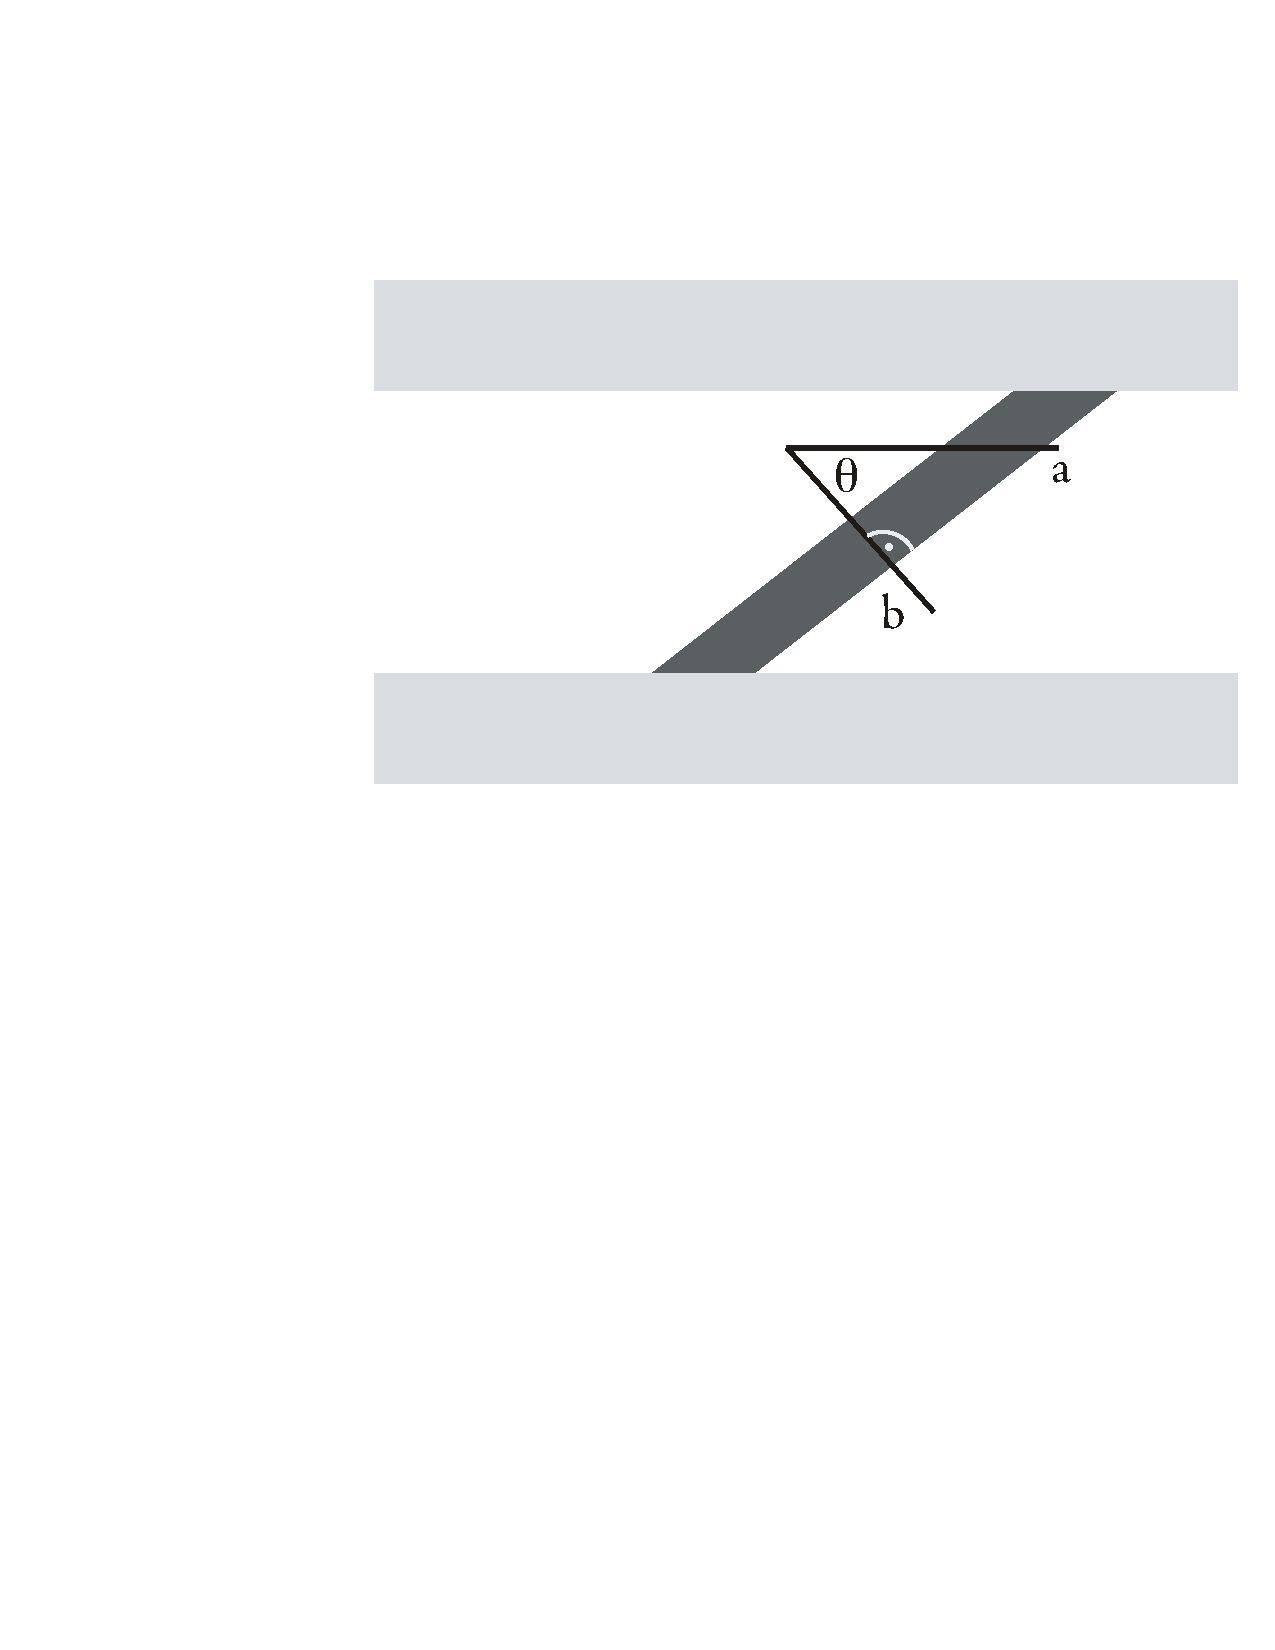
\includegraphics[width=0.6\linewidth]{images/linewidth}
\end{center}
\caption{\label{fig:linewidth}Sketch of line width assessments: (a) is showing the horizontal width, (b) is  width orthogonal to the slope. Participants preferred method (b) over (a).}
\end{figure}

\begin{figure*}[htbp]
\begin{center}
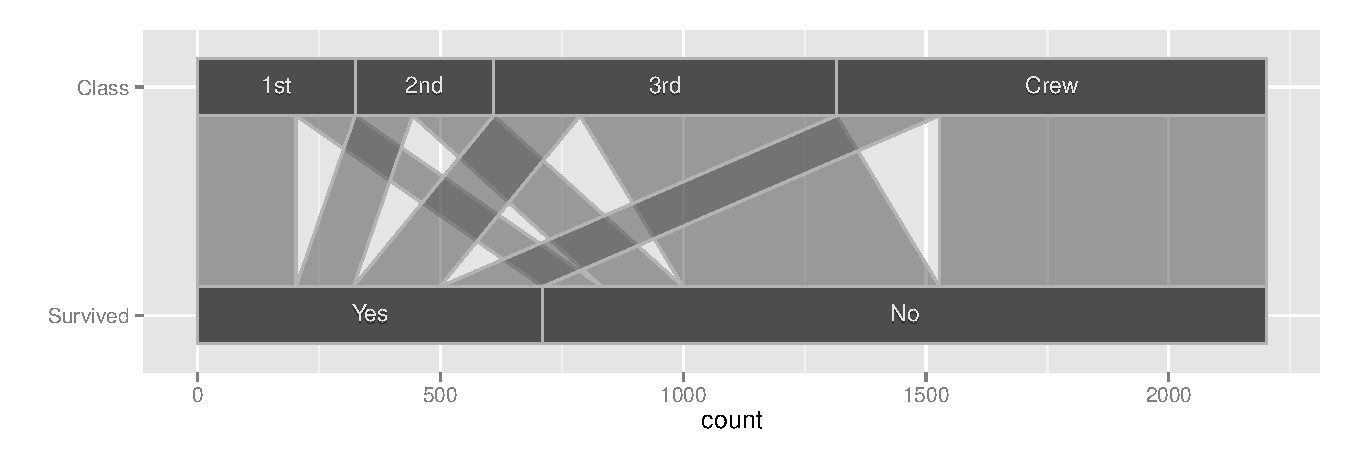
\includegraphics[height=1.5in]{images/aspect31-titanic.pdf}
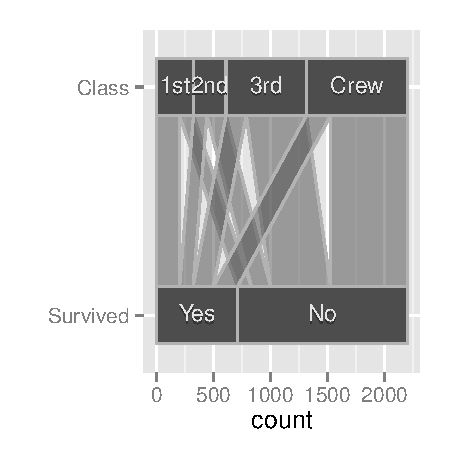
\includegraphics[height=1.5in]{images/aspect33-titanic.pdf}
\end{center}
\caption{\label{fig:aspect}Parallel sets plots of survival on the Titanic by class. Different aspect ratios  seemingly change the (orthogonal) line width, compare e.g. number of survivors in 3rd class and in the crew. }
\end{figure*}

The slope of a line very much depends on the aspect ratio of the corresponding plot - changing the height to width ratio of a display  will change our perception of the corresponding line widths, if they are not adjusted for the slope. Figure \ref{fig:aspect} shows an example for that. The same parallel sets plot is shown twice in this figure, but with very different aspect rations: again, we are looking at survival on the Titanic. In the left plot the number of surviving 3rd class passengers seems to be about twice as big as the number of survivors among crew members, whereas on the right the lines have about equal (orthogonal) width. Obviously, the numbers don't change, but our (intuitive) evaluation of the situation does. Reordering categories, as well as controlling the aspect ratio to avoid huge differences in the slope of lines helps reduce the potential of drawing wrong conclusions from these plot, but none of these measures is enough to avoid all perceptual traps.
% needed in second column of first page if using \IEEEpubid
%\IEEEpubidadjcol
\subsection{Hammock Plots}
%XXX Description of hammock plots and example

Hammock plots \citep{schonlau:2003} provide an alternative to parallel sets that is adjusted for the linewidth illusion by increasing the --horizontal-- linewidth by  a factor of $\sin \theta$, as discussed in equation (\ref{adjust}). This adjusts the perceived --orthogonal-- linewidth to be proportional to the number of observations it represents. 
 Figure \ref{hammock} shows an example of a four dimensional hammock plot of the Titanic data. From top to bottom Class, Gender, Survival, and again Class are shown. 
\begin{figure}
%cols <- c(brewer.pal(name="Blues", 6)[-c(1,2)], rev(brewer.pal(name="Oranges", 3)[-1]), rev(brewer.pal(name="Greens",3)[-1]))
%ggparallel(names(titanic)[c(1,4,2,1)], order=c(0,1,1,0), method="hammock", ratio=.25, text.angle=0, titanic, weight="Freq") +
%  scale_fill_manual(values=cols, guide="none") +
%  scale_colour_manual(values=cols, guide="none") + coord_flip() 
%ggsave("hammock-titanic.pdf", width=6, height=8)
\centering
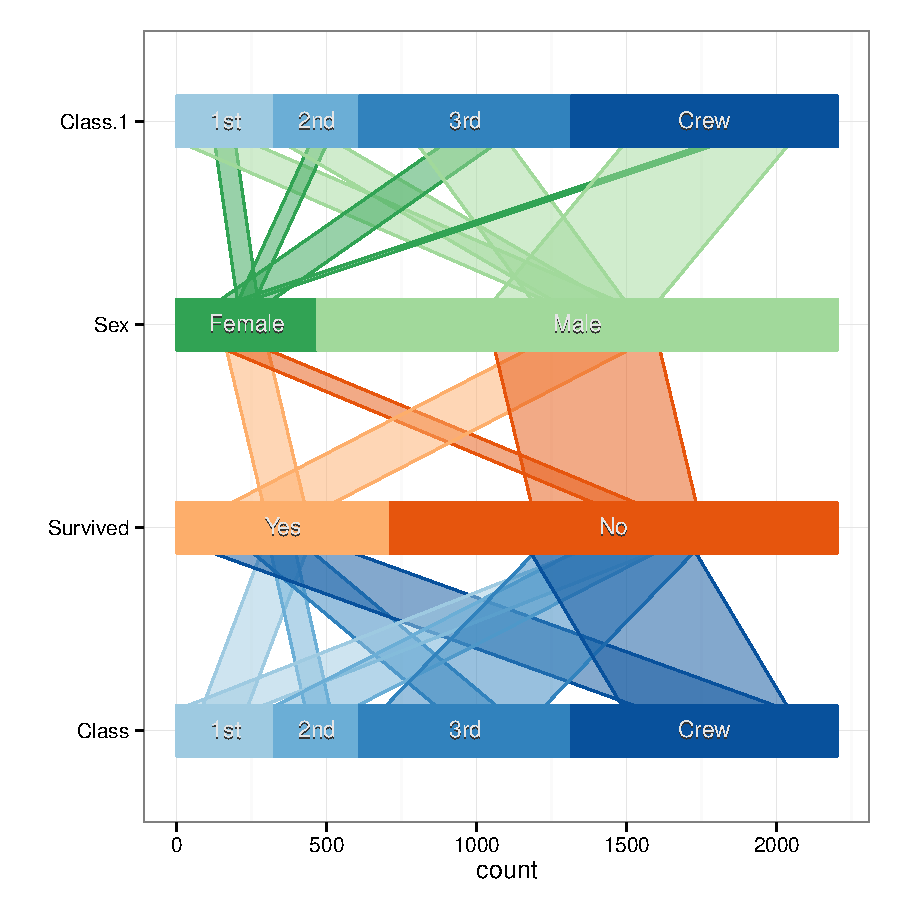
\includegraphics[width=\linewidth]{hammock-titanic}
\caption{\label{hammock} Hammock plot of the Titanic Data. }
\end{figure}

Similar to the parallel sets plot, the bars are divided according to class membership numbers.  Lines connect categories between neighboring bars, line widths are representing the number of individuals in each combination. Unlike the parallel sets, the lines start from the middle of the bin and connect to the middle of the other variable's bin. 
%Line widths are adjusted in such a way, that the orthogonal width (see sketch \ref{fig:linewidth}) represents numbers.

In this example, we see that barely any women were in the crew, while male crew members make up the second largest contingent overall. While a few more men survived than women, proportionally the situation is much different -- a much higher percentage of women survived than men. We also see, that more first class passengers survived than not, while second class passengers survival chances were about fifty-fifty. For third class passengers and crew members fewer members did  survive than not. 

Since the adjustment of line widths is made with respect to the angle $\theta$, which itself depends on the aspect ratio of a plot, we need complete control over these properties of the plotting device when constructing Hammock plots  -- in our implementation (see below for details) we have dealt with this issue by fixing the aspect ratio. This is problematic in some situations, where the rendering has to be done without knowledge of the plotting device. 

Another problem that arises in evaluating hammock plots is that if an observer focuses on horizontal linewidth  the plots suffer from a reverse linewidth illusion:  judging the number of survivors by class in figure \ref{hammock} based on horizontal linewidth would result in in ordering of (largest to smallest ) Crew, 3rd, 1st, and 2nd - which is not correct either. Using horizontal width is inviting, since the lines are centered around the middle of a level, facilitating this  comparison. 

In this paper, we propose a new approach to visualizing categorical variables in a parallel coordinate plot setting, called the {\it common angle} display. 


\section{ Common Angle Plots}
\subsection{Construction}


\begin{figure}[htbp] %  figure placement: here, top, bottom, or page
%ggparallel(names(titanic)[c(1,4,2,1)], order=c(0,1,1,0), titanic, weight="Freq", text.angle=0) + 
%  scale_fill_manual(values=cols, guide="none") +
%  scale_colour_manual(values=cols, guide="none") + coord_flip() 
%ggsave("ca-titanic.pdf", width=6, height=6)
   \centering
   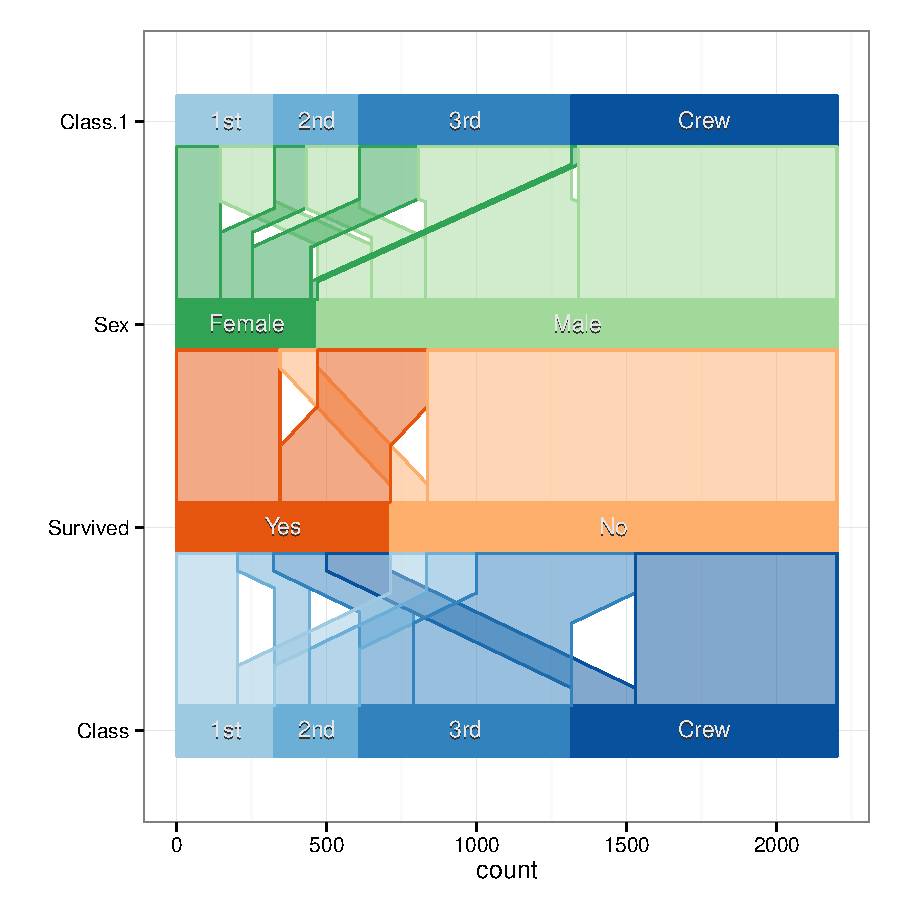
\includegraphics[width=\linewidth]{ca-titanic} 
   \caption{Common Angle plot of the Titanic data. }
   \label{fig:ca-titanic}
\end{figure}

Figure \ref{fig:ca-titanic} shows a common angle plot of the same data as the hammock plot.

As in the previously discussed display types ribbons are drawn between categories with widths  that are proportional to  the number of records they represent.

In order to ensure that their widths are all comparable without any distortion, their slopes  are artificially made the same in the following manner: 
assuming a vertical display as shown in figure \ref{fig:ca-titanic}, we modify  the connecting bands between  categories from a straight band  to a combination of a vertical  segment, a  segment under a pre-specified angle $\theta$, followed by another vertical  segment.  
The pre-specified angle $\theta$ (between the line and the vertical band) is given as --at most-- the angle of the longest connecting line between two categories of neighboring variables. 
This makes the width of ribbons  comparable without being affected by the distortion, since all ribbons are sharing at least one segment under the same angle. 

\subsection{Origins}
Historically, the common angle diagram has its roots in Sankey diagrams \citep{sankey:1898}. Sankey diagrams have their origin and main use of application in the area of industrial engineering. They are often used to show flows,  particularly, in the framework of energy consumption and losses within systems.
One of the most famous charts that can be classified as a Sankey diagram is Minard's map of Napoleon's march on Moscow \citep{minard:1812}. This map  shows the size of the army as a flow chart from West to East and the subsequent retreat back. Usually, Sankey diagrams do not show a geographic co-variate, though. Modern uses of Sankey diagrams are discussed in  detail in \citep{schmidt:2008};  they can also be found in charts designed by Jen Christiansen, such as in \cite{jen1} and \cite{jen2}.

%XXX http://www.jenchristiansen.com/ Jen Christiansen 
%http://jenchristiansen.com/?p=20
%Scientific American references 
%
%Sankey diagrams William O'Brien 'Preliminary Investigation of the use of Sankey diagrams ...'


\subsection{Evaluation}
XXX need IRB modification to allow comparison of common angles, parallel sets and hammock plots

XXX reverse axis for coord\_flip

\section{Applications}
%XXX biological findings - pathways - what are the new findings?
One application using biochemical pathway data is visualization of screening for drug interaction. Setting one bar to classify by pathways and a second bar to classify by physical location (e.g. chromosome), the ribbon widths indicate the number of genes on a particular chromosome that are active in a pathway. A chromosome with ribbons connecting to multiple pathways are a physical target for drugs that possibly affect both paths. In Figure XXX the bottom bar shows two pathways: hsa00232, which is involved in caffeine metabolism, and hsa00982, which is involved with drug metabolism via the cytochrome P450 superfamily. The top bar classifies by chromosome location. Gene CYP1A2 is involved in both pathways - clomipramine (an antidepressant) and caffeine both may act as a substrate.
\begin{figure*}[htbp] %  figure placement: here, top, bottom, or page
   \centering
   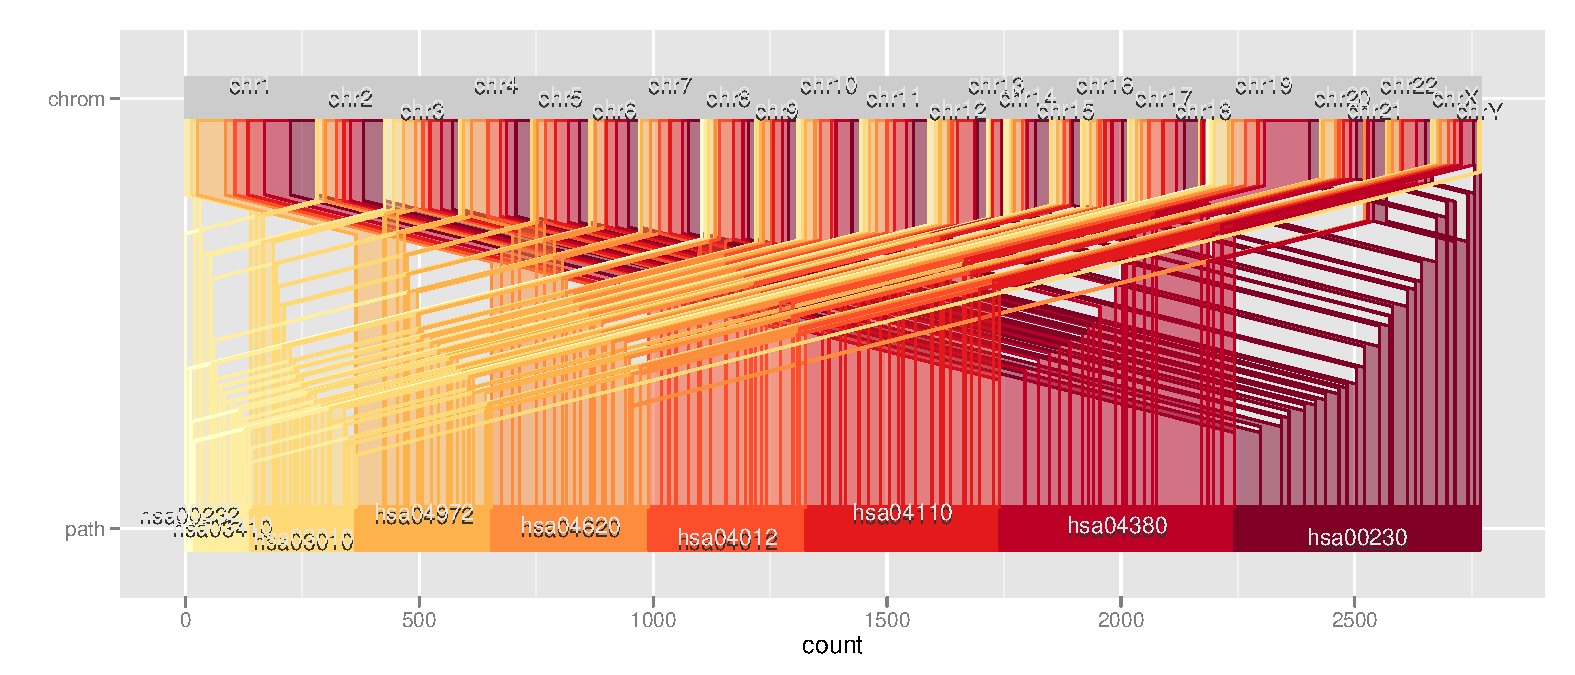
\includegraphics[width=\linewidth]{ca-kegg} 
   \caption{Common angle plot }
   \label{fig:kegg}
\end{figure*}

\begin{figure*}[htbp] %  figure placement: here, top, bottom, or page
   \centering
   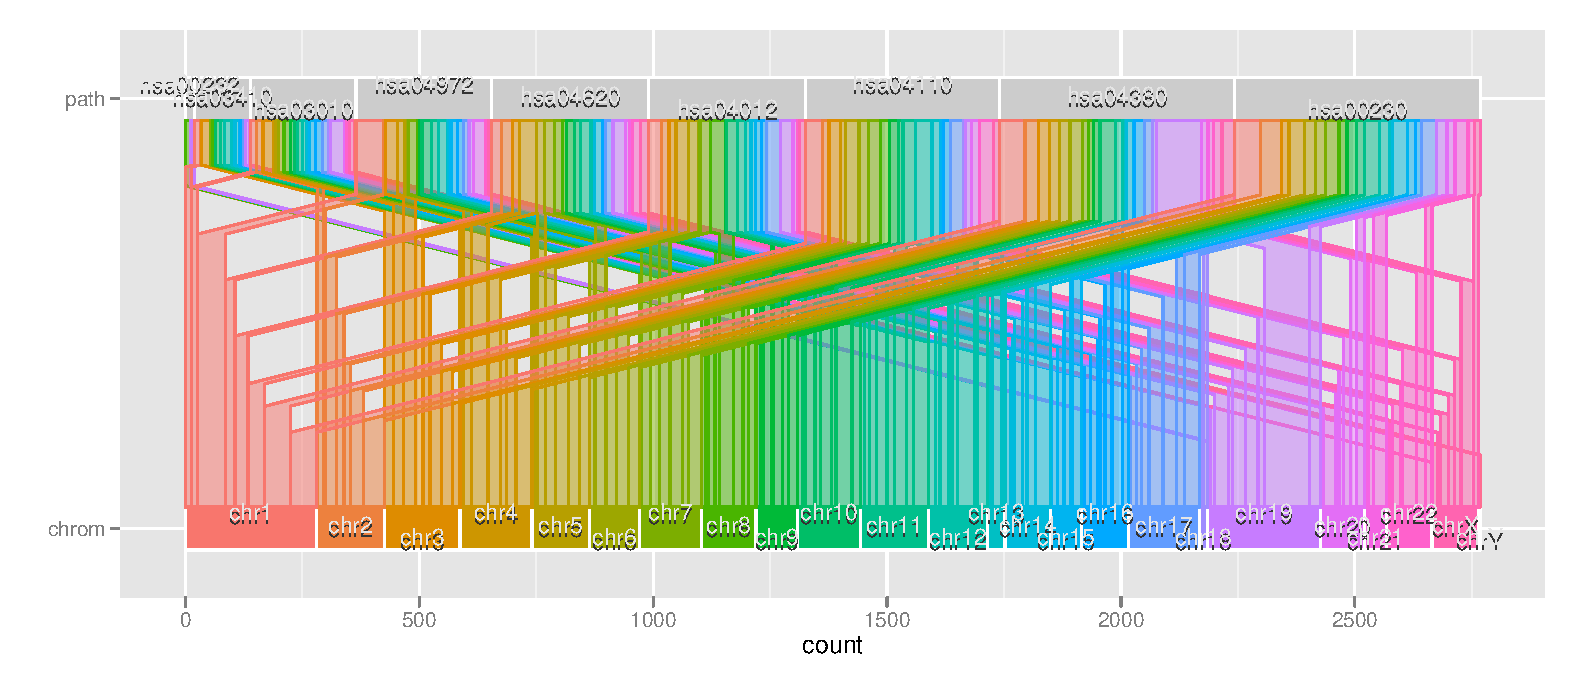
\includegraphics[width=\linewidth]{ca-kegg-2} 
   \caption{Common angle plot }
   \label{fig:kegg:2}
\end{figure*}

\begin{figure*}[htbp] %  figure placement: here, top, bottom, or page
   \centering
   \includegraphics[width=\linewidth]{caffeine_drug} 
   \caption{Common gene activity for caffeine and drug metabolism}
   \label{fig:caffeine}
\end{figure*}


\section{Extensions}
\subsection{Hammock-adjusted common angle plots}
A logical next step in making ribbons comparable across all their parts and multiple variables, we can additionally adjust sloped parts of the ribbons using the hammock-adjustment described above. This leads to a representation as shown in figure \ref{adj.angle}. Ribbons no longer fill the marginal bars. This choice was made to reduce the amount of overplotting resulting from the increase in width of the lines under an angle. Note, that the hammock adjustment results in re-introducing the aspect ratio as a crucial quantity. 
\begin{figure}[hbtp]
%ggparallel(names(titanic)[c(1,4,2,1)], order=c(0,1,1,0), method='adj.angle', text.angle=0, weight="Freq", titanic, ratio=0.035) + 
%  scale_fill_manual(values=cols, guide="none") +
%  scale_colour_manual(values=cols, guide="none") + coord_flip() 
%ggsave("adj-angle.pdf", width=6, height=6)
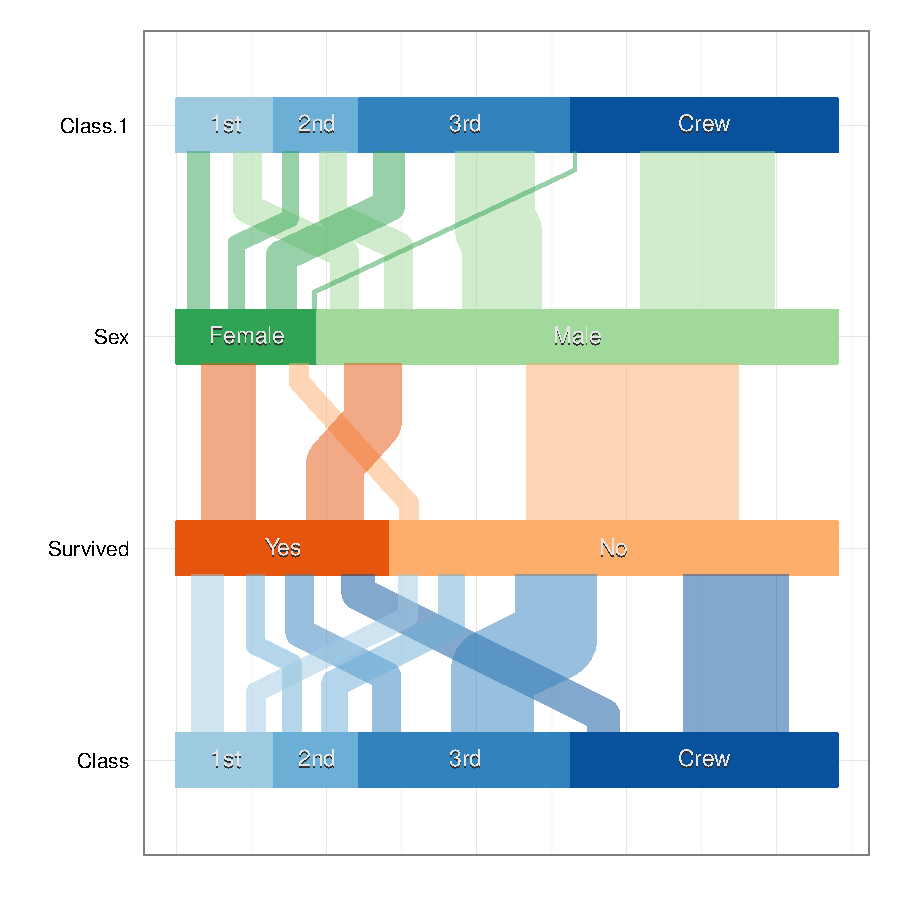
\includegraphics[width=\linewidth]{adj-angle}
\caption{Adjusted common angle plot of the Titanic data.}
\label{adj.angle}
\end{figure}
\section{Implementation}

All  of the discussed variants of parallel coordinate plots for categorical data are implemented as part of the package {\tt ggparallel} based on the {\tt ggplot2} \cite{ggplot2} plotting framework in the software {\tt R} 2.15.1 \citep{R}. The  {\tt ggparallel} package is freely available from CRAN (\url{http://www.r-project.org/}).
The colors for the plots have been chosen using color schemes from the ColorBrewer project  \cite{colorbrewer} , as implemented in the R package {\tt RColorBrewer}  \cite{RColorBrewer} .


\section{Conclusion}
%The conclusion goes here. The conclusion goes here.The conclusion goes here.The conclusion goes here.The conclusion goes here.The conclusion goes here.The conclusion goes here.The conclusion goes here.The conclusion goes here.The conclusion goes here.The conclusion goes here.The conclusion goes here.The conclusion goes here.The conclusion goes here.The conclusion goes here.The conclusion goes here.The conclusion goes here.The conclusion goes here.The conclusion goes here.The conclusion goes here. The conclusion goes here.The conclusion goes here.The conclusion goes here.The conclusion goes here.





% if have a single appendix:
%\appendix[Proof of the Zonklar Equations]
% or
%\appendix  % for no appendix heading
% do not use \section anymore after \appendix, only \section*
% is possibly needed

% use appendices with more than one appendix
% then use \section to start each appendix
% you must declare a \section before using any
% \subsection or using \label (\appendices by itself
% starts a section numbered zero.)
%

%
\appendix
\subsection*{Demographics of the pre-cursory survey I}\label{app1}
33 students, staff and faculty from Iowa State University participated in the survey investigating the strength of the perceptual line width distortion. The Qualtrics system \cite{} was used to create the survey and all students, staff and faculty from programs in Statistics, Bioinformatics and Computational Biology and Human Computer Interaction were invited to participate by email. No personally identifiable information was collected, nor was any compensation offered. Participants used their own personal computing devices to access the survey. A majority of participants used WoW64 (Windows 32-bit or Windows 64-bit), with the next most common operating system Intel Mac OS X10.6.8 (Snow Leopard). The preferred choice of browser was  Chrome, followed by Firefox. 
%No participants chose to do so using internet explorer. 
For two participants, the Qualtrics survey software was unable to capture operating system or browser information.
% ## operating system
% summary(df2$Q2_3_TEXT)
% #                      Intel Mac OS X 10_6_8 Intel Mac OS X 10_7_3   Intel Mac OS X 10.6          Linux x86_64 
% #                    2                     7                     4                     1                     3 
% #               rv:6.0                Ubuntu                 WOW64 
% #                    1                     1                    14 
% 
% ## browser info
% ### NOTE: I discovered after the survey went out that IE renders the html code for the training data poorly
% summary(df2$Q2_1_TEXT)
% #         Chrome Firefox  Safari 
% #      2      16      10       5 

In contrast to that, a second question asking participants to order class levels according to survival {\it rates} of members did not yield any indication that parallel sets were performing less efficiently than barcharts; 11 out of 12 (barcharts) and 12 out of 13 (parallel sets) participants were able to answer this question correctly. The answer was also based on either figure \ref{question1a} or \ref{question1b}. While the line width illusion is present, its effect for this instance is not strong enough to have an impact on the order of the results.



\subsection*{Survey II}\label{app2}
%
%\subsection*{Discussion of Sine Illusion}
%Using the notation given in the applet, we assume a value $s$ for the sine amplitude, $\ell$ for the vertical length of line segments, and $\ell_c$ for the amount of compensation. 
%The sine curve is then given by function $f$, written as 
%\[
%f(x) = s/2 \sin(x)
%\]
%for $x$ in $[-\pi, \pi]$. The slope of the sine curve is the steepest in its reflection point at $x=0$. We can calculate the slope as $f^\prime(x) = s/2 \cos(x)$, which in $x=0$ yields a slope of $s/2$.
%
%The physical dimensions of the applet are 500 pixels by 500 pixels, corresponding to an extent in the $x$ axis of $2 \pi$ and a maximum amplitude and line lengths of 250 in the $y$ axis. This results in an aspect ratio of $250 : (2\pi)$.
%For the physical angle $\theta$ of the slope with respect to the horizontal axis we get
%\[
%\tan \theta =  s/2 \cdot 2\pi/250 = s\pi/250
%\]
%Adding a compensation of $\ell_c$ to the length of line segments is supposed to make the orthogonal width of the region of the steepest slope appear as wide as the vertical length in the turning point. Since the slope in the turning point is zero, the extent of the width is unchanged and is therefore equal to $\ell$. 
%We therefore get for an `optimal' compensation as
%\[
%\ell \stackrel{!}{=} \cos \theta \cdot \left( \ell + \ell_c \right),
%\]
%yielding 
%\[
%\ell_c = \left(1 - \cos \theta\right)/\cos \theta \ \  \ell.
%\]
%theta <- function(s) atan(s*pi/250)
%compensate <- function(theta) (1-cos(theta))/cos(theta)



% use section* for acknowledgement
\ifCLASSOPTIONcompsoc
  % The Computer Society usually uses the plural form
  \section*{Acknowledgments}
\else
  % regular IEEE prefers the singular form
  \section*{Acknowledgment}
\fi


All surveys for this study were carried out with approval from  IRB-ID 12-204.


% Can use something like this to put references on a page
% by themselves when using endfloat and the captionsoff option.
\ifCLASSOPTIONcaptionsoff
  \newpage
\fi



% trigger a \newpage just before the given reference
% number - used to balance the columns on the last page
% adjust value as needed - may need to be readjusted if
% the document is modified later
%\IEEEtriggeratref{8}
% The "triggered" command can be changed if desired:
%\IEEEtriggercmd{\enlargethispage{-5in}}

% references section

% can use a bibliography generated by BibTeX as a .bbl file
% BibTeX documentation can be easily obtained at:
% http://www.ctan.org/tex-archive/biblio/bibtex/contrib/doc/
% The IEEEtran BibTeX style support page is at:
% http://www.michaelshell.org/tex/ieeetran/bibtex/
\bibliographystyle{IEEEtran}
% argument is your BibTeX string definitions and bibliography database(s)
\bibliography{references}
%
% <OR> manually copy in the resultant .bbl file
% set second argument of \begin to the number of references
% (used to reserve space for the reference number labels box)
%\begin{thebibliography}{1}
%
%\bibitem{IEEEhowto:kopka}
%%This is an example of a book reference
%H. Kopka and P.W. Daly, \emph{A Guide to {\LaTeX}}, third ed. Harlow, U.K.: Addison-Wesley, 1999.
%
%
%%This is an example of a Transactions article reference
%%D.S. Coming and O.G. Staadt, "Velocity-Aligned Discrete Oriented Polytopes for Dynamic Collision Detection," IEEE Trans. Visualization and Computer Graphics, vol.?14,? no.?1,? pp. 1-12,? Jan/Feb? 2008, doi:10.1109/TVCG.2007.70405.
%
%%This is an example of a article from a conference proceeding
%%H. Goto, Y. Hasegawa, and M. Tanaka, "Efficient Scheduling Focusing on the Duality of MPL Representation," Proc. IEEE Symp. Computational Intelligence in Scheduling (SCIS '07), pp. 57-64, Apr. 2007, doi:10.1109/SCIS.2007.367670.
%
%%This is an example of a PrePrint reference
%%J.M.P. Martinez, R.B. Llavori, M.J.A. Cabo, and T.B. Pedersen, "Integrating Data Warehouses with Web Data: A Survey," IEEE Trans. Knowledge and Data Eng., preprint, 21 Dec. 2007, doi:10.1109/TKDE.2007.190746.
%
%%Again, see the IEEEtrans_HOWTO.pdf for several more bibliographical examples. Also, more style examples
%%can be seen at http://www.computer.org/author/style/transref.htm
%\end{thebibliography}

% biography section
% 
% If you have an EPS/PDF photo (graphicx package needed) extra braces are
% needed around the contents of the optional argument to biography to prevent
% the LaTeX parser from getting confused when it sees the complicated
% \includegraphics command within an optional argument. (You could create
% your own custom macro containing the \includegraphics command to make things
% simpler here.)
%\begin{biography}[{\includegraphics[width=1in,height=1.25in,clip,keepaspectratio]{mshell}}]{Michael Shell}
% or if you just want to reserve a space for a photo:

\begin{IEEEbiography}{Heike Hofmann}
Biography text here.
\end{IEEEbiography}

\begin{IEEEbiography}{Marie Vendettuoli}
Biography text here.
\end{IEEEbiography}

% if you will not have a photo at all:
%\begin{IEEEbiographynophoto}{John Doe}
%Biography text here.Biography text here.Biography text here.Biography text here.Biography text here.Biography text here.Biography text here.Biography text here.Biography text here.Biography text here.Biography text here.Biography text here.Biography text here.Biography text here.Biography text here.Biography text here.Biography text here.Biography text here.Biography text here.Biography text here.Biography text here.Biography text here.Biography text here.Biography text here.Biography text here.Biography text here.Biography text here.Biography text here.Biography text here.Biography text here.Biography text here.Biography text here.
%\end{IEEEbiographynophoto}
%
%% insert where needed to balance the two columns on the last page with
%% biographies
%%\newpage
%
%\begin{IEEEbiographynophoto}{Jane Doe}
%Biography text here.Biography text here.Biography text here.Biography text here.Biography text here.Biography text here.Biography text here.Biography text here.Biography text here.Biography text here.Biography text here.Biography text here.Biography text here.Biography text here.Biography text here.Biography text here.Biography text here.Biography text here.Biography text here.Biography text here.Biography text here.Biography text here.Biography text here.Biography text here.Biography text here.Biography text here.Biography text here.Biography text here.
%\end{IEEEbiographynophoto}

% You can push biographies down or up by placing
% a \vfill before or after them. The appropriate
% use of \vfill depends on what kind of text is
% on the last page and whether or not the columns
% are being equalized.

%\vfill

% Can be used to pull up biographies so that the bottom of the last one
% is flush with the other column.
%\enlargethispage{-5in}



% that's all folks